\documentclass[../../main.tex]{subfiles}

\begin{document}

\section{Motivation}

Convolutional Neural Networks (CNNs) are a class of neural networks that are renowned for be translation equivariant, they have been widely used in image processing tasks and have shown to be able to learn spatial patterns in the data via convolutional filters. CNNs are very powerful and have been the state of the art in many image processing tasks making them a desirable backbone for a Neural Process. Hence, the motivation for Convolutional Neural Processes (ConvCNPs) \parencite{gordon2020convolutional}. We will breifly discuss the ConvCNP model and its architecture however for a more detailed explanation, we refer the reader to the original paper.

\section{Model}

\begin{figure}[H]
	\centering
	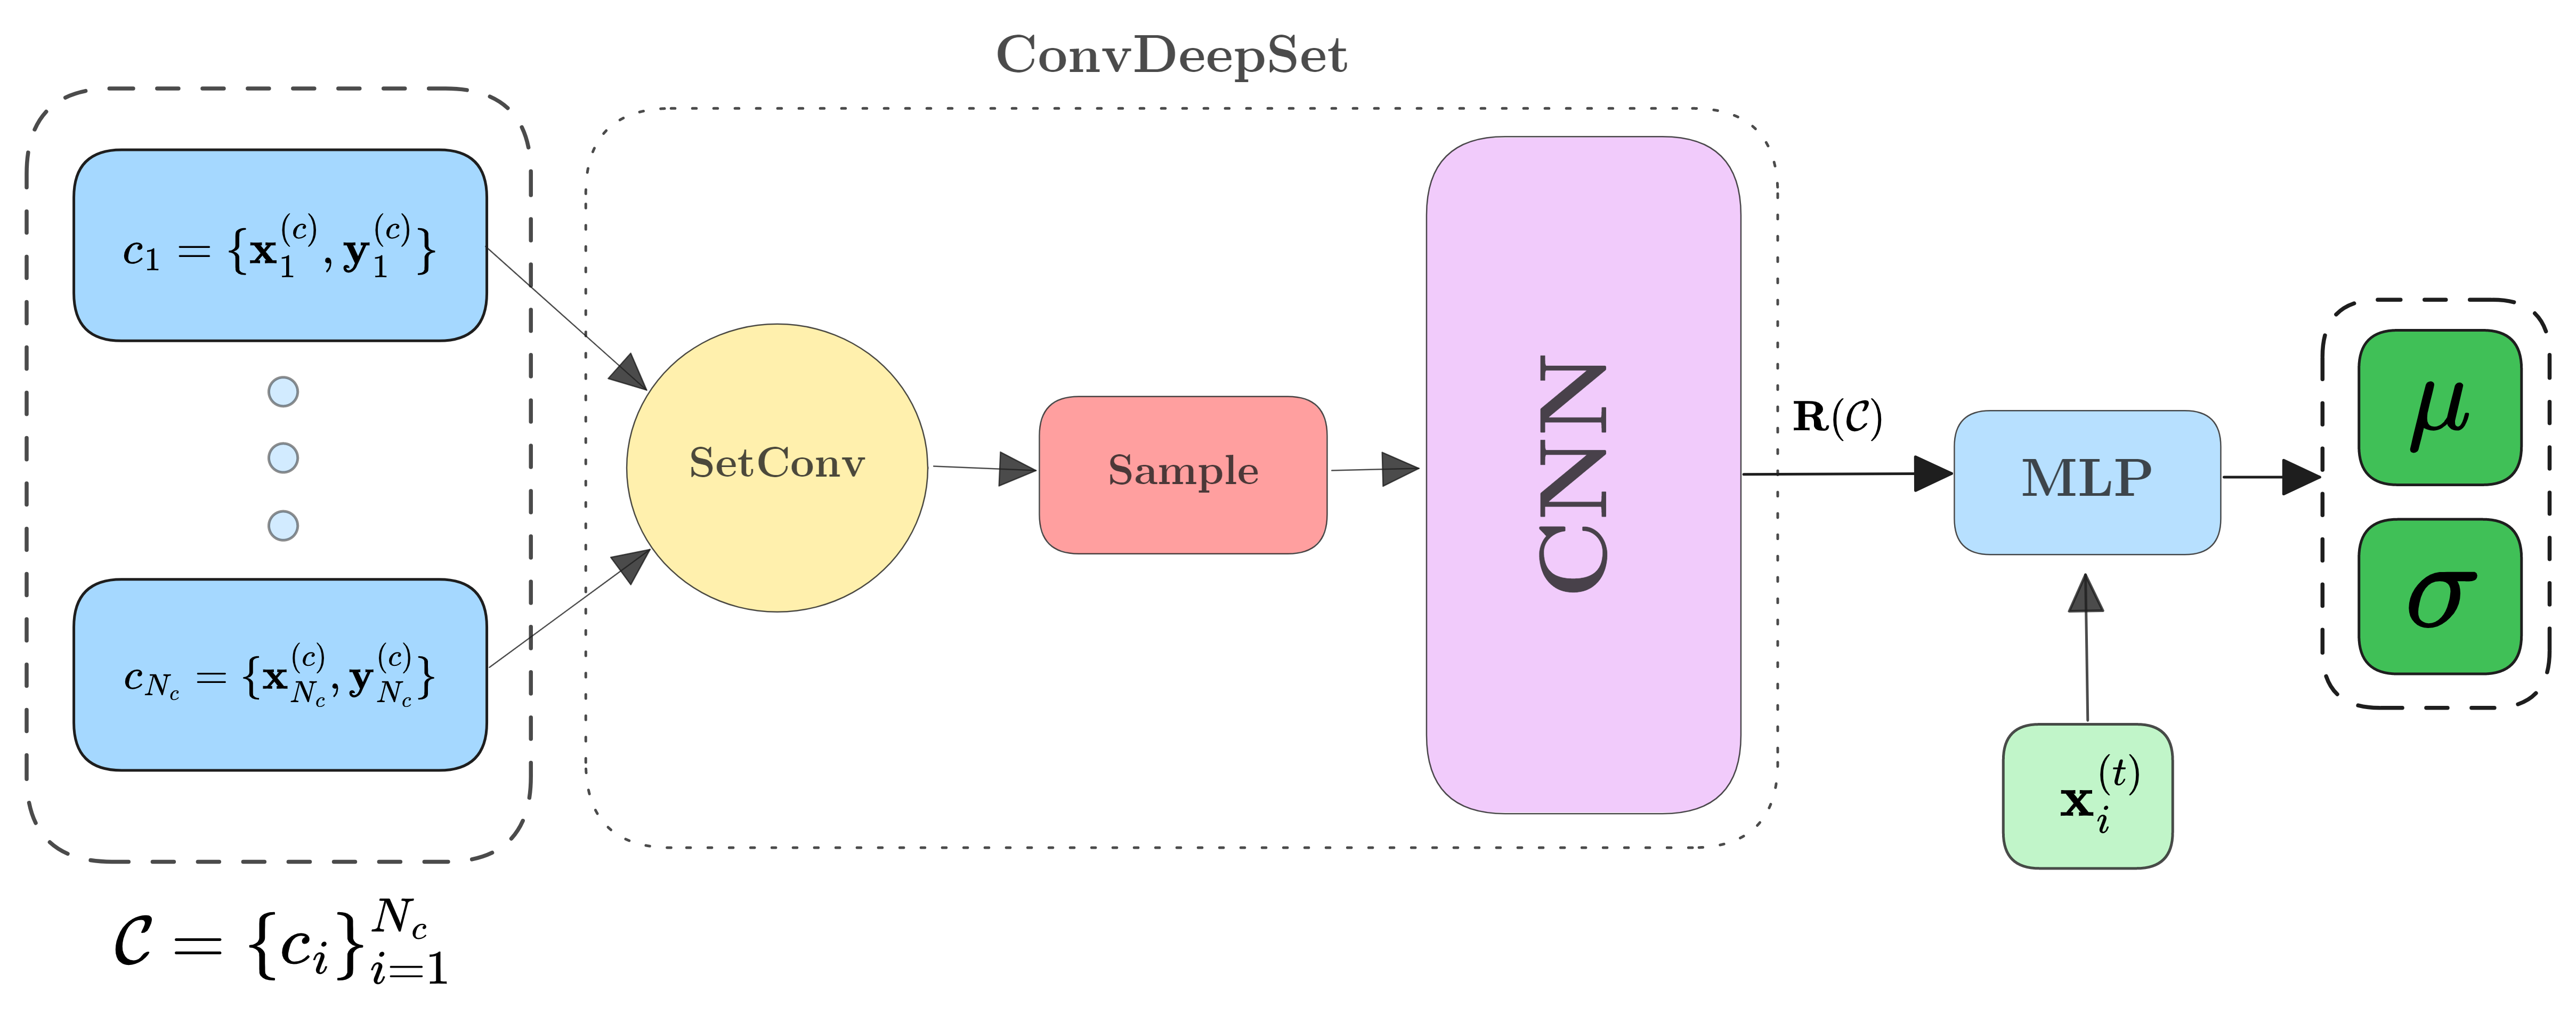
\includegraphics[width=0.8\textwidth]{convcnp.png}
	\caption{ConvCNP Architecture}
	\label{fig:convcnp}
\end{figure}


ConvCNPs \parencite{gordon2020convolutional} \autoref{fig:convcnp} utilize CNNs, more specifically the UNet architecture. However, a few hurdles are preventing us from directly plugging data into a CNN.


CNNs operate on \textbf{on-grid data}, meaning that the data is on a regular grid, for example, an image. However, the data we are working with is sometimes \textbf{off-grid data}, for example time series dataset with irregular timestamps. Furthermore, to `bake-in' the TE property, we need to be able to shift the data in the input space and the output space in the same way. This is not trivial when using standard vector representations of the data. \parencite{gordon2020convolutional} propose a solution to this problem by using \textbf{functional embeddings} to model the data. Functional embeddings are a way to represent data as a function that has a trivial translation equivariance property. 


These functional embeddings are created using the \textbf{SetConv} operation. The SetConv operation is a generalization of the convolution operation that operates on sets of data, it takes a set of input-output pairs and outputs a continuous function. The SetConv operation is defined as follows:
\begin{equation}
	\text{SetConv}(\{\bm{x_i}, \bm{y_i}\}_{i=1}^{N})(x) = \sum_{i=1}^{N} [1, \bm{y_i}] ^ T \mathcal{K}(\bm{x} - \bm{x_i})
\end{equation}

Where $\mathcal{K}$ is a kernel function that measures the distance between the query $x$ and the data point $\bm{x_i}$.

This operation has some key properties:
\bul{
	\item We append $1$ to output $\bm{y_i}$ when computing the SetConv, this acts as a flag to the model so that it knows which data points are observed and which are not. Say we have a data point of $\bm{y_i} = 0$, then if we did not append the $1$, the model would not be able to distinguish between an observed data point and an unobserved data point (as both would be $0$).
	\item The `weight' of the Kernel depends only on the relative distance between points on the input space which means that the model is translation equivariant.
	\item The summation over the data points naturally introduces \textbf{Permutation Invariance} to the model, meaning that the order of the data points does not matter.
}

In \parencite{gordon2020convolutional}, they refer to the addition of the $1$ as the \textbf{density channel}, this channel is used to distinguish between observed and unobserved data points. 

% \todo{Take figure from the ConvCNP paper to show functional embeddings}

Now that we have a function representation of the context set, we need to sample it/discretize it at \textbf{evenly} spaced points. Thus converting the data into a \textbf{on-grid} format. Now it can be fed into a CNN. Now that we have a CNN that operates on the data, we need to convert it back to a continuous function. This is done again by using the \textbf{SetConv} operation. The final output of the encoder is a continuous function that represents the context set which can be queried at any point in the input space using the target set.

\begin{equation}
	R(\bm{x_t}) = \text{SetConv}(\text{CNN}(\{\text{SetConv}(\mathcal{C})(\bm{x_d})\}_{d=1}^{D}))(\bm{x_t})
\end{equation}



The decoder is a simple MLP that takes the output of the encoder and the target set as input and outputs the mean and variance of the predictive distribution $\bm{\mu}(\bm{x_t}), \bm{\sigma}(\bm{x_t}) = \text{MLP}(R(\bm{x_t}))$


\ifSubfilesClassLoaded{%
    \printbibliography{}
}{} 


\end{document}